%%% Add comments with at least three %%% preceding.
%%% Add new sections with one % preceding
%%% Add new subsections with two %% preceding

\def\dllpk     {\ensuremath{\mathrm{DLL}_{\proton\kaon}}\xspace}

%%%%%%%%%%%%%
% Non standard particles
%%%%%%%%%%%%%
% light vectors
\ifthenelse{\boolean{uprightparticles}}%
{\def\Prho      {\ensuremath{\uprho}\xspace}
 \def\Pphi      {\ensuremath{\upphi}\xspace}
}
{\def\Prho      {\ensuremath{\rho}\xspace}
 \def\Pphi      {\ensuremath{\phi}\xspace}
}
\def\rhoz   {\ensuremath{\Prho^0}\xspace}
\def\rhozs  {\ensuremath{\Prho^0\mbox\,\rm{s}}\xspace}
\def\rhop   {\ensuremath{\Prho^+}\xspace}
\def\rhom   {\ensuremath{\Prho^-}\xspace}
\def\phiz   {\ensuremath{\Pphi^0}\xspace}
\def\phizs  {\ensuremath{\Pphi^0\mbox\,\rm{s}}\xspace}
\def\had  {\ensuremath{\Ph}\xspace}
\def\hadp  {\ensuremath{\Ph^+}\xspace}
\def\hadm  {\ensuremath{\Ph^-}\xspace}
\def\hadpm  {\ensuremath{\Ph^{\pm}}\xspace}
\def\hadmp  {\ensuremath{\Ph^{\mp}}\xspace}
\def\hadprim  {\ensuremath{\had^{\prime}}\xspace}
\def\hadprimp  {\ensuremath{\had^{\prime+}}\xspace}
\def\hadprimm {\ensuremath{\had^{\prime-}}\xspace}
\def\hadprimpm  {\ensuremath{\had^{\prime\pm}}\xspace}
\def\hadprimmp  {\ensuremath{\had^{\prime\mp}}\xspace}

\def\pipi  {\ensuremath{\pip\pim}\xspace}
\def\KpKm  {\ensuremath{\Kp \kern -0.16em \Km}\xspace}
\def\KzKzb {\ensuremath{\Kz \kern -0.16em \Kzb}\xspace}

% heavy vectors
\def\Bdz      {\ensuremath{\Bd}\xspace}
\def\Bsz      {\ensuremath{\Bs}\xspace}
\def\Bdsz      {\ensuremath{\Bz_{(\squark)}}\xspace}
\def\Dpstarz  {\ensuremath{\D^{(*)0}}\xspace}
\def\Dpstarzb {\ensuremath{\Dbar^{(*)0}}\xspace}
\def\Dpstarm  {\ensuremath{\D^{(*)-}_{\squark}}\xspace}
\def\Dpstarp {\ensuremath{\Dbar^{(*)+}_{\squark}}\xspace}
\def\Lbz  {\ensuremath{\Lb^{0}}\xspace}
\def\Lcm  {\ensuremath{\Lc^{-}}\xspace}

\def\kpi       {\ensuremath{\kaon\pion}\xspace}
\def\kk      {\ensuremath{\Kp\Km}\xspace}
\def\kppim     {\ensuremath{\Kp\pim}\xspace}
\def\kmppipm   {\ensuremath{\Kmp\pipm}\xspace}
\def\kmppipmpiz   {\ensuremath{\Kmp\pipm\piz}\xspace}
\def\kmppipmpipmpimp {\ensuremath{\Kmp\pipm\pipm\pimp}\xspace}
\def\kmpip     {\ensuremath{\Km\pip}\xspace}

\def\mumu      {\ensuremath{\mup\mun}\xspace}

\def\pp    {\ensuremath{\proton\proton}\xspace}
\def\ppbar    {\ensuremath{\proton\antiproton}\xspace}

%%%%%%%%%%%%%
% Decays
%%%%%%%%%%%%%
% B decays (charmless)
\def\BdtoKzKK   {\decay{\Bd}{\Kz \Kp \Km}}
\def\BdtoKzPiPi   {\decay{\Bd}{\Kz \pip \pim}}
\def\BdtoKzKPi   {\decay{\Bd}{\Kz \Kpm \pimp}}

\def\BstoKzKK   {\decay{\Bs}{\Kz \Kp \Km}}
\def\BstoKzPiPi   {\decay{\Bs}{\Kz \pip \pim}}
\def\BstoKzKPi   {\decay{\Bs}{\Kz \Kpm \pimp}}

\def\BdstoKzKK   {\decay{\Bdsz}{\Kz \Kp \Km}}
\def\BdstoKzPiPi   {\decay{\Bdsz}{\Kz \pip \pim}}
\def\BdstoKzKPi   {\decay{\Bdsz}{\Kz \Kpm \pimp}}

\def\BdtoKsKK   {\decay{\Bd}{\KS \Kp \Km}}
\def\BdtoKsPiPi   {\decay{\Bd}{\KS \pip \pim}}
\def\BdtoKsKPi   {\decay{\Bd}{\KS \Kpm \pimp}}

\def\BstoKsKK   {\decay{\Bs}{\KS \Kp \Km}}
\def\BstoKsPiPi   {\decay{\Bs}{\KS \pip \pim}}
\def\BstoKsKPi   {\decay{\Bs}{\KS \Kpm \pimp}}

\def\BdstoKsKK   {\decay{\Bdsz}{\KS \Kp \Km}}
\def\BdstoKsPiPi   {\decay{\Bdsz}{\KS \pip \pim}}
\def\BdstoKsKPi   {\decay{\Bdsz}{\KS \Kpm \pimp}}

\def\Kshh{\ensuremath{\KS \hadp \hadm}\xspace}
\def\Kshhp{\ensuremath{\KS \hadp \hadprimm}\xspace}
\def\KshhpSS{\ensuremath{\KS \hadp \hadprimp}\xspace}

\def\KsPiPi{\ensuremath{\KS \pip \pim}\xspace}
\def\KsKPi{\ensuremath{\KS \Kpm \pimp}\xspace}
\def\KsKK{\ensuremath{\KS \Kp \Km}\xspace}
\def\KsPiP{\ensuremath{\KS \pip \antiproton}\xspace}

\def\BdtoKshhp   {\decay{\Bd}{\KS \hadp \hadprimm}}
\def\BdtoKshh   {\decay{\Bd}{\KS \hadp \hadm}}

\def\BstoKshhp   {\decay{\Bs}{\KS \hadp \hadprimm}}
\def\BstoKshh   {\decay{\Bs}{\KS \hadp \hadm}}

\def\BdstoKshhp   {\decay{\Bdsz}{\KS \hadp \hadprimm}}
\def\BdstoKshh   {\decay{\Bdsz}{\KS \hadp \hadm}}

\def\BdtoKPiPiz {\decay{\Bd}{\Kp \pim \piz}}
\def\BstoKPiPiz {\decay{\Bs}{\Km \pip \piz}}

\def\BdtoetapKs   {\decay{\Bdz}{\etapr (\to \rhoz \gamma) \KS}}
\def\ButoDzKtoKsPiPi {\decay{\Bu}{\Dz(\to \KS \pip \pim) \Kp}}
\def\ButoDzPitoKspipi {\decay{\Bu}{\Dz(\to \KS \pip \pim) \pip}}
\def\ButoDzPitoKsKK   {\decay{\Bu}{\Dz(\to \KS \Kp \Km) \pip}}
\def\ButoDstpitoKSPiPi   {\decay{\Bu}{\Dpstarzb(\to \Dzb (\to \KS \pip \pim) \piz ) \pip}}
\def\BdtoKsPiPiGamma   {\decay{\Bdz}{\KS \pip \pim \gamma}}
\def\ButoKsPiPiPi   {\decay{\Bu}{\KS \pip \pim \pip}}
\def\BdtoKstzrhoztoKsPizPiPi   {\decay{\Bdz}{\Kstarz (\to \KS \piz) \rhoz (\to \pip \pim)}}
\def\BstoKstzPhiztoKsPizKK   {\decay{\Bsz}{\Kstarz (\to \KS \piz) \Pphi (\to \Kp \Km)}}
\def\BstoKstKstbartoKsPizKPi   {\decay{\Bsz}{\Kstarz (\to \KS \piz) \Kstarzb (\to \Km \pip)}}
\def\LbtoDsstptoKsPip    {\decay{\Lbz}{\Dpstarm (\to \Dsm (\to \KS \Km)\gamma ) \proton}}

% B decays (charmed, charmonia)
\def\BdtoPsisChicKs {\decay{\Bd}{(\jpsi,\psitwos,\chic) \KS}}
\def\BdtoPsiKstoMuMu {\decay{\Bd}{\jpsi(\to \mup \mun) \KS}}
\def\BdtoPsitwosKs {\decay{\Bd}{\psitwos \KS}}
\def\BdtoPsisKs {\decay{\Bd}{\jpsi(\psitwos) \KS}}
\def\BdtoDmhptoKshm {\decay{\Bd}{\Dm(\to \KS \hadm) \hadp}}
\def\BstoDsmhptoKshm {\decay{\Bs}{\Dsm(\to \KS \hadm) \hadp}}
\def\BstoDsmKp {\decay{\Bs}{\Dsm \Kp}}
\def\ButoDsth {\decay{\Bu}{\Dstarm \hadp}}
\def\ButoDzKtoKsPiPi {\decay{\Bu}{\Dz(\to \KS \pip \pim) \Kp}}
\def\ButoDzPitoKspipi {\decay{\Bu}{\Dz(\to \KS \pip \pim) \pip}}
\def\ButoDzPitoKsKK   {\decay{\Bu}{\Dz(\to \KS \Kp \Km) \pip}}
\def\ButoDstpitoKSPiPi   {\decay{\Bu}{\Dpstarzb(\to \Dzb(\to \KS \pip \pim) \piz ) \pip}}
\def\LbtoDsstptoKsPip    {\decay{\Lbz}{\Dpstarm (\to \Dsm (\to \KS \Km)\g ) \proton}}
\def\LbtoDsmptoKshm    {\decay{\Lbz}{\Dsm(\to \KS \hadm) \proton}}
\def\LbtoDsmptoKsPim    {\decay{\Lbz}{\Dsm(\to \KS \pim) \proton}}
\def\LbtoLcPitoKspb    {\decay{\Lbz}{\Lcm(\to \KS \antiproton) \pip}}

% b decays
\def\btou    {\decay{\bquark}{\uquark}}
\def\btoc    {\decay{\bquark}{\cquark}}
\def\btos    {\decay{\bquark}{\squark}}
\def\btod    {\decay{\bquark}{\dquark}}

\def\btoqqbars {\decay{\bquark}{\quark\quarkbar\squark}}
\def\btossbars {\decay{\bquark}{\squark\squarkbar\squark}}
\def\btoccbars {\decay{\bquark}{\cquark\cquarkbar\squark}}

%%%%%%%%%%%%%
% Reconstruciton mode of KS
%%%%%%%%%%%%%
\def\LL   {Long\xspace}
\def\DD   {Downstream\xspace}

%%%%%%%%%%%%%
% Dalitz variables
%%%%%%%%%%%%%
\newcommand{\mPrime}{\ensuremath{\m^{\prime}}\xspace}
\newcommand{\thPrime}{\ensuremath{\theta^{\prime}}\xspace}


%%%%%%%%%%%%%
% sPlots
%%%%%%%%%%%%%
%\newcommand{\splot}{\hbox{$_s$}${\cal P}$lot\xspace}


%%%%%%%%%%%%%
% Branching fractions
%%%%%%%%%%%%%
\newcommand{\Br}[1]{\ensuremath{\BF\left(#1\right)}\xspace}
\def\fsfd {\ensuremath{\frac{f_{\squark}}{f_{\dquark}}}\xspace}
\def\fsfdinline {\ensuremath{f_{\squark}/f_{\dquark}}\xspace}

%%%%%%%%%%%%%
% Lumis
%%%%%%%%%%%%%
\newcommand{\intlumfb}[1]{\ensuremath{\intlum{#1}\,\invfb}}
\newcommand{\intlumpb}[1]{\ensuremath{\intlum{#1}\,\invpb}}


%%%%%%%%%%%%%
% Commands
%%%%%%%%%%%%%
\newcommand{\eq}[1]{Eq.~\ref{equation : #1}}
\newcommand{\eqs}[2]{Eqs.~\ref{equation : #1}-\ref{equation : #2}}
\newcommand{\tab}[1]{Table~\ref{tab : #1}}
\newcommand{\tabs}[2]{Tables~\ref{tab : #1}-\ref{tab : #2}}
\newcommand{\tabstwo}[2]{Tables~\ref{tab : #1} and~\ref{tab : #2}}
\newcommand{\fig}[1]{Fig.~\ref{fig : #1}}
\newcommand{\figfull}[1]{Figure~\ref{fig : #1}}
\newcommand{\figstwo}[2]{Figs.~\ref{fig : #1} and~\ref{fig : #2}}
\newcommand{\figstwofull}[2]{Figures~\ref{fig : #1} and~\ref{fig : #2}}
\newcommand{\figs}[2]{Figs.~\ref{fig : #1}-\ref{fig : #2}}
\newcommand{\figsfull}[2]{Figures~\ref{fig : #1}-\ref{fig : #2}}
\newcommand{\ttst}[1]{\textrm{\scriptsize{#1}}}
\newcommand{\refsec}[1]{Sect.~\ref{sec : #1}}



%%%%%%%%%%%%%
% Categories
%%%%%%%%%%%%%
\def\TIS   {\texttt{L0TIS}\xspace}
\def\TOS   {\texttt{L0TOSOnly}\xspace}
\def\HltOne   {\texttt{Hlt1TOS}\xspace}
\def\HltOneTwo   {\texttt{Hlt(1,2)TOS}\xspace}

%%%%%%%%%%%%%
% Fit parameters
%%%%%%%%%%%%%
\newcommand{\fitMeanBd}{\ensuremath{\mu_{\Bd}\xspace}}
\newcommand{\fitMeanBs}{\ensuremath{\mu_{\Bs}\xspace}}


%%%%%%%%%%%%%
% Packages
%%%%%%%%%%%%%

\def\bender    {\mbox{\textsc{Bender}}\xspace}

\def\argus {ARGUS\xspace}




\section{CP Violation}
\label{sec:cpv}

The discovery of Physics Beyond the Standard Model (BSM) is the main target of
current high energy experiments. One way to search for this ``New Physics'' is
to measure precisely some parameters which are precisely predicted by the
theory. In this respect, CP violation is particularly interesting because in
the SM, it originates from a single parameter. All the CP violating
observables in the $K$, $B$ and $D$ meson sectors are thus directly related and
their combined study provides a highly powerful test of the whole SM dynamics.
Indeed, most model of New Physics are far less restrictive and allow for a
plethora of new CP-violating sources. None of the delicate interplays between
observables expected in the SM should survive to the presence of new dynamics
at the~TeV scale.

When experimentally testing SM predictions, it is fundamental that the
theoretical precision matches the experimental accuracy. A priori, this looks
challenging because CP-violation is a purely hadronic phenomenon in the SM,
originating from the quark couplings. However, dedicated strategies have been
designed and CP-violating observables are actually among our best windows. For
example, in CP-violating asymmetries, most of the uncertainties cancel between
the numerator and the denominator, so that we can construct measurable
quantities with small uncertainties. Alternatively, some observables are
predicted to be so small that they can be considered forbidden in the SM, and
simply observing a non-zero value would unequivocally signal the presence of
New Physics.

The French community has been deeply involved in CP-violation experiments for
many years (CPLEAR, NA48, BaBar, LHCb, ...). Expertise has been developed in
several key aspects of CP-violation: amplitude analyses, tagged-time-dependent
angular analyses, flavour tagging, neutral objects, ... More specifically, the
French community has been involved in the measurements of the Unitarity angles
$\alpha$, $\gamma$ and $\phi_{s}$. Among other decay channels, the following
have been
studied in detail:
$B_{(s,d)}\to D^{0} K^{*0}$, $B_{(s,d)}\to\bar{D}^{0} hh$, $B^{0}_{s} \to
D_{s} K$, $B^{0}_{s} \to J/\psi\phi$,
$B^{0}_{s} \to J/\psi\bar{K}^{*0}$. 
Other studies, of $b$ hadrons to charmless final states will be commented in
Sec.~\ref{sec:charmless}.
One of the outcome of the work done is
$\phi_{s}$ is illustrated on Figure~\ref{figphis}.
% $B^{0}\to\rho\rho$, $B_{(s,d)}\to K^{0}_{\mathrm{S}} hh$, $B^{0} \to K^{0}_{\mathrm{S}} K \pi$,

Expertise has also been acquired on designing, building and maintaining key
elements of the detectors: trigger and calorimeters.

%+ PCI40, SciFi
%CPLEAR, NA48, NA62, BaBar, LEP(?) LHCb

In the coming years, most of the experimental effort will go in LHCb and its
upgrade plans. One of the biggest challenge will be to store and analyse the
enormous quantity of data from the LHC.

%CHRISTOPHER>
From the theory side, ... CKMfitter, QCD challenge, precision challenge,
sub-leading diagram estimation, penguin pollution, ...

In the 4 following years (2017-2020), we will not only continue the
measurements started many years ago, with the full run2 data-set of the LHC,
but also explore new routes:

\begin{itemize}
\item several ways to measure $\gamma$ and $\alpha$;

\item continue efforts on $\phi_{s}$ and control of sub-leading penguins contributions;

\item explore CP violation in baryons;

\item CP violation in charm is still to be discovered.

\item CP violation in kaon: Are we planning to perform some lattice studies,
for example of the $\varepsilon^{\prime}$ matrix elements? Also, theorists are
certainly following closely the NA62 experiment which aims at $K^{+}%
\rightarrow\pi^{+}\nu\nu$.

\item EDM: should we include the nEDM experiment? It is among the IN2P3 projects.
\end{itemize}

For all these items, the synergy between experimental and theoretical
communities is essential, because a major discovery can not come if the
uncertainties are not under control in both places.

We will also actively participate to the brainstorming on future upgrade of
the LHCb experiment, i.e. plans for the 2025-2035 period.

\begin{figure}[!htb]
\begin{center}
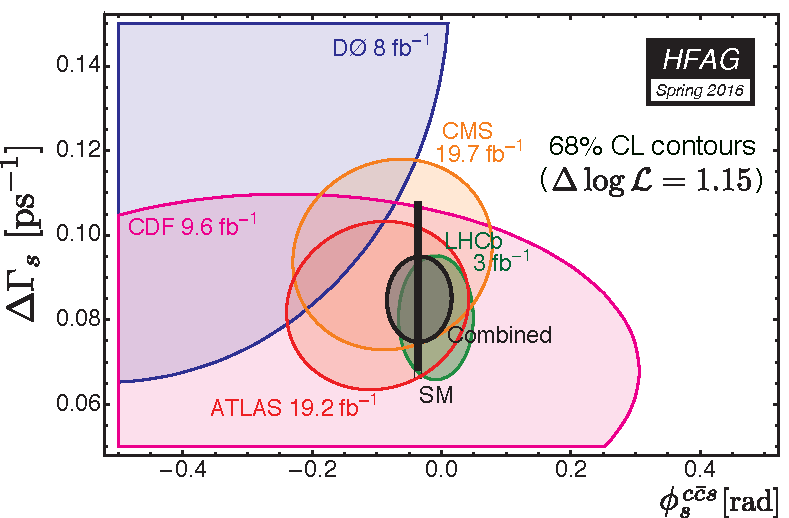
\includegraphics[width=10cm]{hfag_Spring2016_DGsphis_zoom.pdf}
\end{center}
\caption{68\% CL regions in $B^{0}_{s}$ width difference $\Delta\Gamma_{s}$
and weak phase $\phi_{s}$ obtained from individual and combined CDF, D0,
ATLAS, CMS and LHCb likelihoods of $B^{0}_{s}\to J/\psi\phi$, $B^{0}_{s}\to
J/\psi KK$, $B^{0}_{s}\to J\psi\pi\pi$ and $B^{0}_{s}\to D_{s}^{+}D_{s}^{-}%
$.The expectation within the Standard Model is shown as the black rectangle.}%
\label{figphis}%
\end{figure}





\section{Charmless $b$ Hadron Decays}
\label{sec:charmless}

The study of of $b$-hadron decays to hadronic final states with no charmed particles allow for a rich array of studies. A few examples are the measurements of branching fractions, CP asymmetries, weak and strong phases and the CKM angles; they probe the dynamics of weak and strong interactions. The typical branching fractions of these modes are below $10^{-5}$ and thus their analyses are feasible only with large data samples and the use of powerful tools to reject background. The LHCb experiment is an adequate experimental environment for these analyses, offering the possibility to study decays of light $B$ mesons, $B_s$ mesons and $b$ baryons.

In particular, CP-violation related studies of charmless $b$-hadron decays have a number of theoretical applications and that provide a probe to new physics, along the lines described in Sec.~\ref{sec:cpv}.
For instance, the decays \BdtoKsPiPi and \BdtoKsKK are dominated by \btoqqbars ($q = u,d,s$)
loop transitions.
Mixing-induced \CP asymmetries in such decays are predicted to be approximately
equal to those in \btoccbars transitions, \eg $\Bd\to\jpsi\KS$, by the
Cabibbo-Kobayashi-Maskawa mechanism~\cite{Cabibbo:1963yz,Kobayashi:1973fv}.
However, the loop diagrams that dominate the charmless decays can have
contributions from new particles in several extensions of the Standard Model,
which could introduce additional weak phases~\cite{Buchalla:2005us,Grossman:1996ke,London:1997zk,Ciuchini:1997zp}.
A time-dependent analysis of the three-body Dalitz plot allows measurements of
the mixing-induced \CP-violating
phase~\cite{Dalseno:2008wwa,Aubert:2009me,Nakahama:2010nj,Lees:2012kxa}. 
 The current experimental measurements of \btoqqbars decays~\cite{HFAG} show
fair agreement with the results from \btoccbars decays (measuring the weak
phase \Pbeta) for each of the scrutinised \CP eigenstates.
There is, however, a global trend towards lower values than the weak phase
measured from \btoccbars decays.
The interpretation of this deviation is made complicated by QCD
corrections, which depend on the final state~\cite{Silvestrini:2007yf} and
are difficult to handle.
An analogous extraction of the mixing-induced \CP-violating phase in the
\Bs system ($\beta_s$) will, with a sufficiently large dataset, also be possible with
the \BstoKsKPi decay, which can be compared with that from, \eg
$\Bs\to\jpsi\phi$.

An impressive harvest of results from charmless hadronic $B$ mesons decays was obtained by the $B$ factories. Several french groups participated in these studies within the BaBar experiment, and in particular, a part of the present LPNHE-LHCb group. The LHCb experiment is already playing an important role in this area of physics, with the participation of the LPC and LPNHE groups. Both have contributed to the LHCb analysis of the decay modes \BstoKshhp ($\had^{(\prime)} = \pi, K$) with $1$~fb$^{-1}$ of data, which are being pursued with $3$~fb$^{-1}$.  In particular they are performing amplitude analyses (aka Dalitz-plot analyses) of \BdtoKsPiPi and \BdtoKsKK decays. At LHCb, the first step of the charmless $b$ hadron decays physics programme is to establish the signals of yet unobserved rare modes. The only yet-unobserved \BstoKshhp mode is \BstoKsKK. The LPC group also performs analyses of $B_s \to \rho^0 \rho^0$, and $\Lambda_b^0 (\Xi_b^0) \to p \had \had^{\prime}\had^{\prime\prime}$ decays.

All the analyses mentioned above provide a long-term physics programs that can profit from the LHCb upgrade. These analyses proceed in increasingly complex steps, which become more and more sensitive to new physics observables with the growing dataset, and with more observed decay modes. One of the long-term goals is to perform full flavor- and time-dependent Dalitz-plot analyses of the \BstoKshhp modes to the measure the weak phases $\beta$ and $\beta_s$. Recent theoretical and experimental activity has focused on the determination of the CKM angle \Pgamma from charmless $B$ meson decays using and refining the methods proposed in Refs.~\cite{Ciuchini:2006kv,Gronau:2006qn,Bhattacharya:2013cla}. The LPNHE group is checking the applicability of the method described in the last reference to the LHCb physics analysis. Moreover, with the upgrade of LHCb, more modes, eventually with more neutral hadrons, are being considered.